\subsection{El aspecto de energías no renovables}

Las principales fuentes de energía con las que cuenta hoy el mundo, petróleo, gas natural y carbón mineral, son de carácter no renovable o convencional; es decir que a medida que se van consumiendo disminuyen sus reservas sin posible reposición, salvo que se descubran nuevos yacimientos.\\

Este sector de energías convencionales sigue teniendo un papel protagónico en la matriz energética mundial, producto de un mercado con muchos años de desarrollo tecnológico, con un gran capital hundido en infraestructura, costos competitivos y con porcentajes de rendimiento y de potencia firme superiores a las renovables. Sin embargo, el consumo de combustibles de origen fósil tiene un efecto muy negativo para el medio ambiente, ya que el dióxido de carbono que se produce por su combustión es el principal constituyente de lo que se conoce como gases de efecto invernadero, principales responsables del calentamiento global.\\

Las consecuencias de este efecto son, por ejemplo, el aumento de las temperaturas, los picos de temperaturas extremos, que han venido manifestándose en los últimos años. Es por ello, que las emisiones globales de carbono continúan aumentando, lo que indica la necesidad de un conjunto integral de medidas políticas para lograr la reducción sustancial de las emisiones de carbono.\\

\begin{figure}[H]
    \centering
    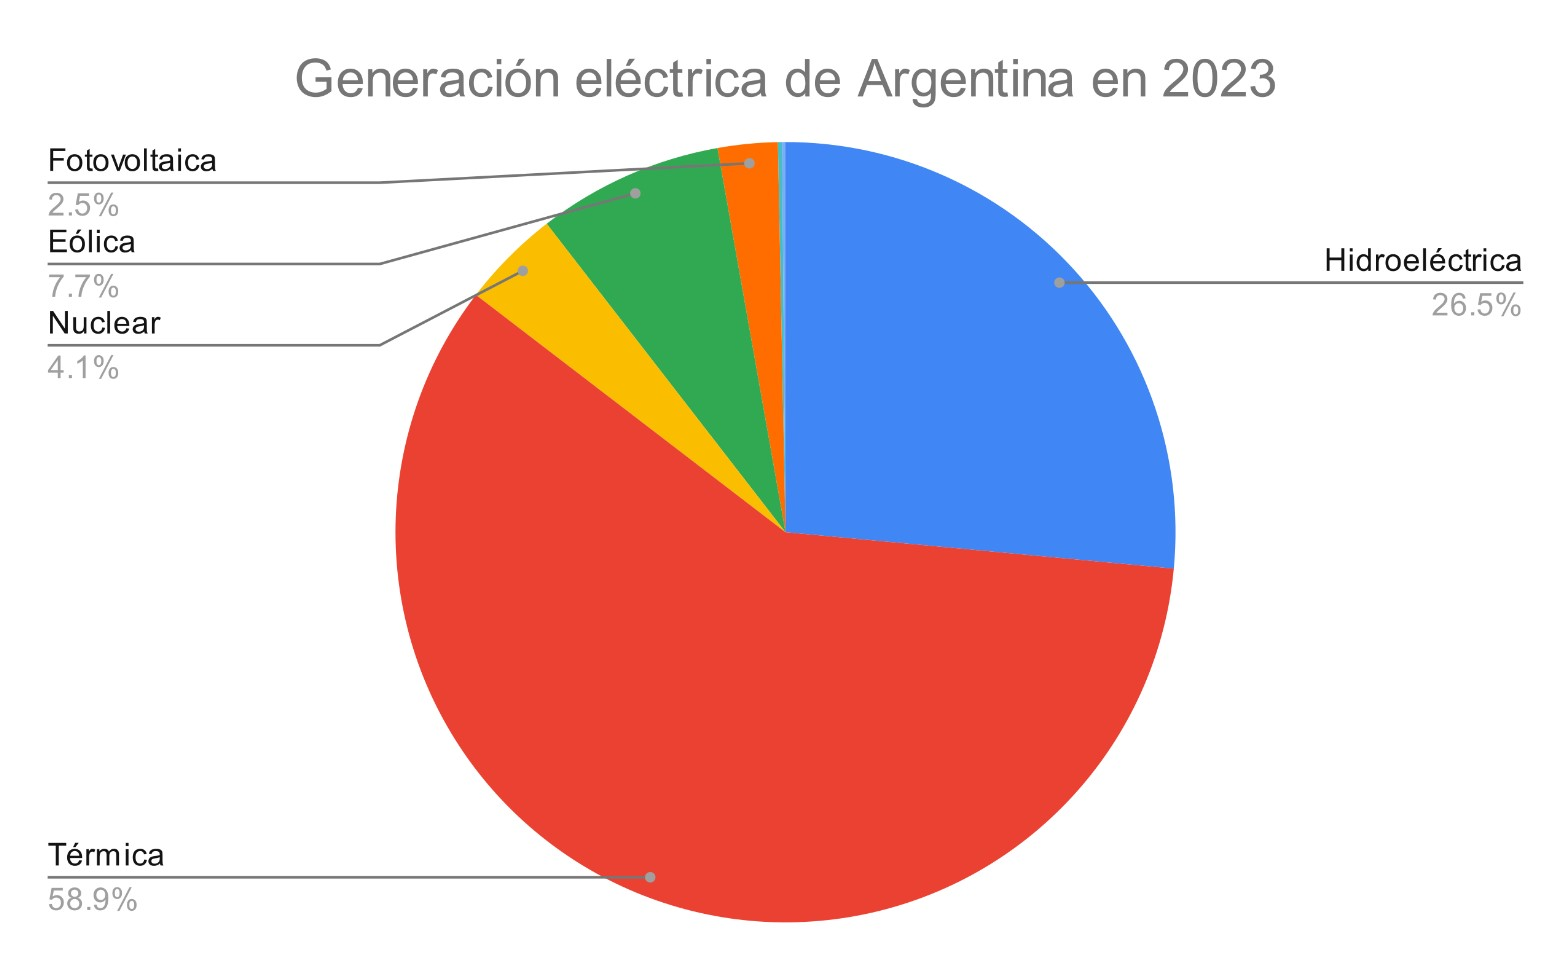
\includegraphics[width=0.85\linewidth]{ambiente/Screenshot_20.jpg}
    \caption{Matriz de generación energética en Argentina}
    \label{fig:matriz-energias}
\end{figure}

En Argentina, casi el 60\% de la energía producida y distribuida en el país son de carácter no renovable. La visión de Solar Link es aportar a que ésta brecha vaya disminuyendo hasta su exterminacion, volviendo a las energias renovables cabecillas en la generacion de energia. \\

\subsection{Uso de baterías en la actualidad}
En la actualidad, las baterías de litio están tomando cada vez mas protagonismo en el mercado. Estas, luego de su uso, se vuelven obsoletas y generan desechos que no son reciclables, sin contar que su extracción es altamente nociva y genera residuos contaminantes. \\

La solución que nosotros proponemos es impulsar el uso de baterías de plomo ácido, que no solo son reciclables hasta en un 80\%, sino que tienen una expectativa de vida mayor. Esto sumado al cargador MPPT de Solar Link, que maximiza el potencial recibido de una fuente de energía renovable y la vida útil de las baterías, creemos que es una solución tanto viable como económica. \\

\subsection{El aspecto de la energía solar}
El sol es el mayor suministro de energía que dispone la humanidad disponible de forma ilimitada
y que puede ser aprovechada en cualquier parte del mundo. Existen dos maneras principales de capturar esta energía solar: la fotovoltaica y la térmica, ambas comparten la virtud que pueden ser producidas y consumidas en cualquier lugar, tanto en áreas remotas o grandes ciudades.\\

En las economías emergentes, como la Argentina, donde existe déficit de infraestructura en
generación, transporte y distribución, esta energía permite soluciones de generación a los
individuos o poblaciones aisladas.

\begin{figure}[H]
\centering
\begin{subfigure}{0.4\textwidth}
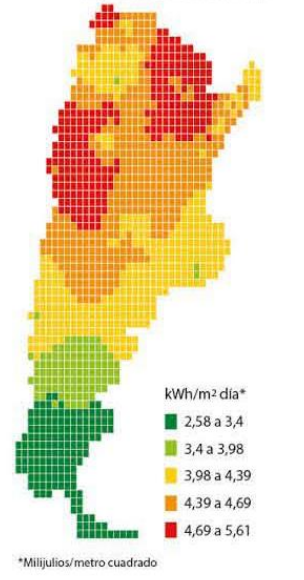
\includegraphics[width=1\linewidth]{ambiente/Screenshot_1.png} 
\caption{Zonas del pais con mayor \\promedio de intensidad de \\radiación solar}
\end{subfigure}
\begin{subfigure}{0.4\textwidth}
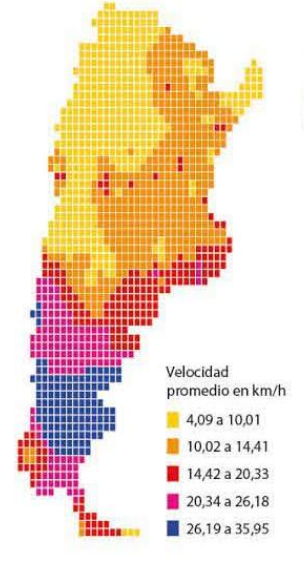
\includegraphics[width=1\linewidth]{ambiente/Screenshot_2.png}
\caption{Zonas del pais con mayor \\promedio de intensidad de \\los vientos}
\label{fig:subim2}
\end{subfigure}
\label{fig:image2}
\end{figure}

Nótese que justamente las provincias con más potencial solar (inclusive eólico) son aquellas donde el consumo de energía eléctrica es mucho más caro en comparación con el gran Bs As y otros centros urbanos, principalmente por los altos costos de distribución de energía. Acá es donde Solar Link tendría su mayor aprovechamiento.\\

Considerando la estadística mostrada, un metro cuadrado de panel solar (en bs as) podría generar 4 kW/h por día. Suponiendo que el panel está en uso 12hs por día, se generan 330 W/h por metro cuadrado de panel. 
En realidad, los paneles son menos eficientes que esto, por tanto para recibir esos 330W/h los paneles son más grandes que 1 metro cuadrado. \\
Sabiendo esto, usaremos como ejemplo un panel solar de 380 W/h y 1.75 metros cuadrados. Por tanto durante, en promedio, 12 hs, se recibirán 380 W/h en el panel. Esta generación de energía implica que por día se producen 4.56 kW/h.\\

En promedio, por mes, una casa de núcleo familiar consume 600 kW/h, o sea 20 kW/h por día. Si hacemos números, nos da que el sistema sería capaz de alimentar con energía solar el 25\% de esa carga (en promedio), ya que de los 600 kW/h por mes, 140 pudieron generarse con el sistema para cargar las baterías y que estas después alimenten las líneas competentes. \\

Hoy en dia el desarrollo de la tecnologia relacionado con la energía solar crece exponencialmente, haciendo mas barato y accesible estos sistemas. A su vez, en argentina disminuye el subsidio destinado a la distribución eléctrica, cerrando lentamente la brecha monetaria entre pagar la luz y recurrir a energias renovables. \\

Teniendo en cuenta todo lo dicho anteriormente, el uso de energias renovables no solo se esta volviendo plausible, sino que tambien se esta volviendo rentable y accesible. Nuestro objetivo con Solar Link es volver esta esperanza en una realidad. \\